%!TEX root = ../main.tex
%%%%%%%%%%%%%%%%%%%%%%%%%%%%%%%%%%
% Links:
%
% Difficulty:
% Companies: 
%%%%%%%%%%%%%%%%%%%%%%%%%%%%%%%%%%

\chapter{Trapping Water}
\label{ch:trapping_water}
\section*{Introduction}
This chapter describes a quite challenging and extremely popular and fun problem that is asked at big companies like Google and Microsoft. 


\section{Problem statement}
\begin{exercise}
Write a function that takes as input an array of length $n$ of non-negative integers representing an elevation map (or an histogram) where the width of each bar is $1$. The function should return the amount of water that is trapped in the histogram after an heavy rain overnight. 

	\begin{example}
		\label{ex:trapping_water:exmaple1}
		\hfill \\
		Given the array $H=[0,1,0,2,1,0,1,3,2,1,2,1]$ (see Figure \ref{fig:trapping_water_example1}), the function return $8$
	\end{example}

	\begin{example}
		\label{ex:trapping_water:exmaple2}
		\hfill \\
		Given the array $H=[1,0,2,1,0,1]$ (see Figure \ref{fig:trapping_water_example2}), the function return $14$
	\end{example}

\end{exercise}

\begin{figure}
		\label{fig:trapping_water_example1}
		\centering
		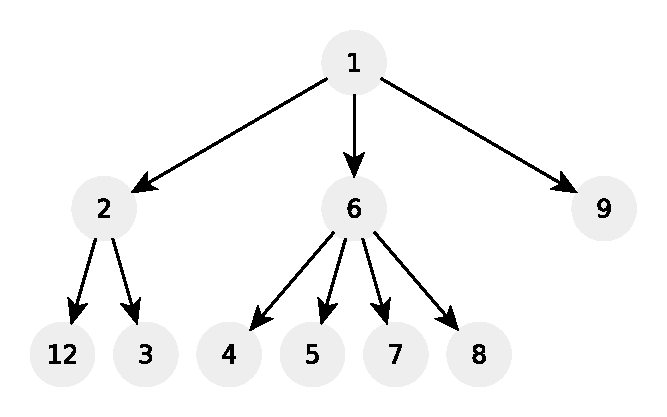
\includegraphics[scale=1.0]{/home/dspataro/git/algorithm_articles/sources/trapping_water/images/example1}
		\caption{Visual representation of the example \ref{ex:trapping_water:exmaple1}. Blue squares represent water, while the red ones, bricks.}
\end{figure}



\begin{figure}
		\label{fig:trapping_water_example2}
		\centering
		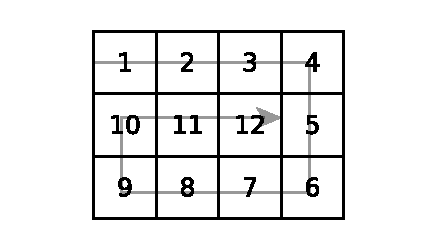
\includegraphics[scale=1.0]{/home/dspataro/git/algorithm_articles/sources/trapping_water/images/example2}
		\caption{Visual representation of the example \ref{ex:trapping_water:exmaple2}. Blue squares represent water, while the red ones, bricks.}
\end{figure}

%\section{Clarification Questions}
%
%\begin{QandA}
%	\item 
%	\begin{answered}
%		\textit{}
%	\end{answered}
%	
%\end{QandA}

\section{Discussion}
\label{trapping_water:sec:discussion}
There are at least $3$ of ways we can solve this challenge in a way that will satisfy our interviewer:

\begin{enumerate}
	\item Dynamic programming
	\item Stack based solution
	\item Two pointers
\end{enumerate}
We will start investigating this problem by using a brute force approach, for then to pass on more sophisticated and better solutions.


\subsection{Brute-force}
\label{trapping_water:sec:bruteforce}

The brute-force approach is easy once we realize that each element of the array can potentially be holding some water provided that there are other two bars, one on its left and one on its right, with height equal or higher than its. It that is the case then, we can safely add enough water so the its level reach the minimum between the highest bar on the left and on the right.
For instance w.r.t. to \ref{ex:trapping_water:exmaple2}, we can see that for the element at index $6$ having height $1$, the highest bars on its left and right sides are both respectively of height $3$ and $4$. We can fill with water the boxes at index $6$ up to an height of $3$ (the minimum between $3$ and $4$).
If the current element is higher than both the highest bars on its left and right side, then it is not possible to fit any water on it (for instance, this is the case when processing the highest bar on the histogram).  Figure \ref{fig:trapping_water_example3} depicts how one element (the one marked with the question mark) of the array can be processed using this approach i.e. by calculating the minimum between $b_l$ and $b_r$.


\begin{figure}
		\label{fig:trapping_water_example3}
		\centering
		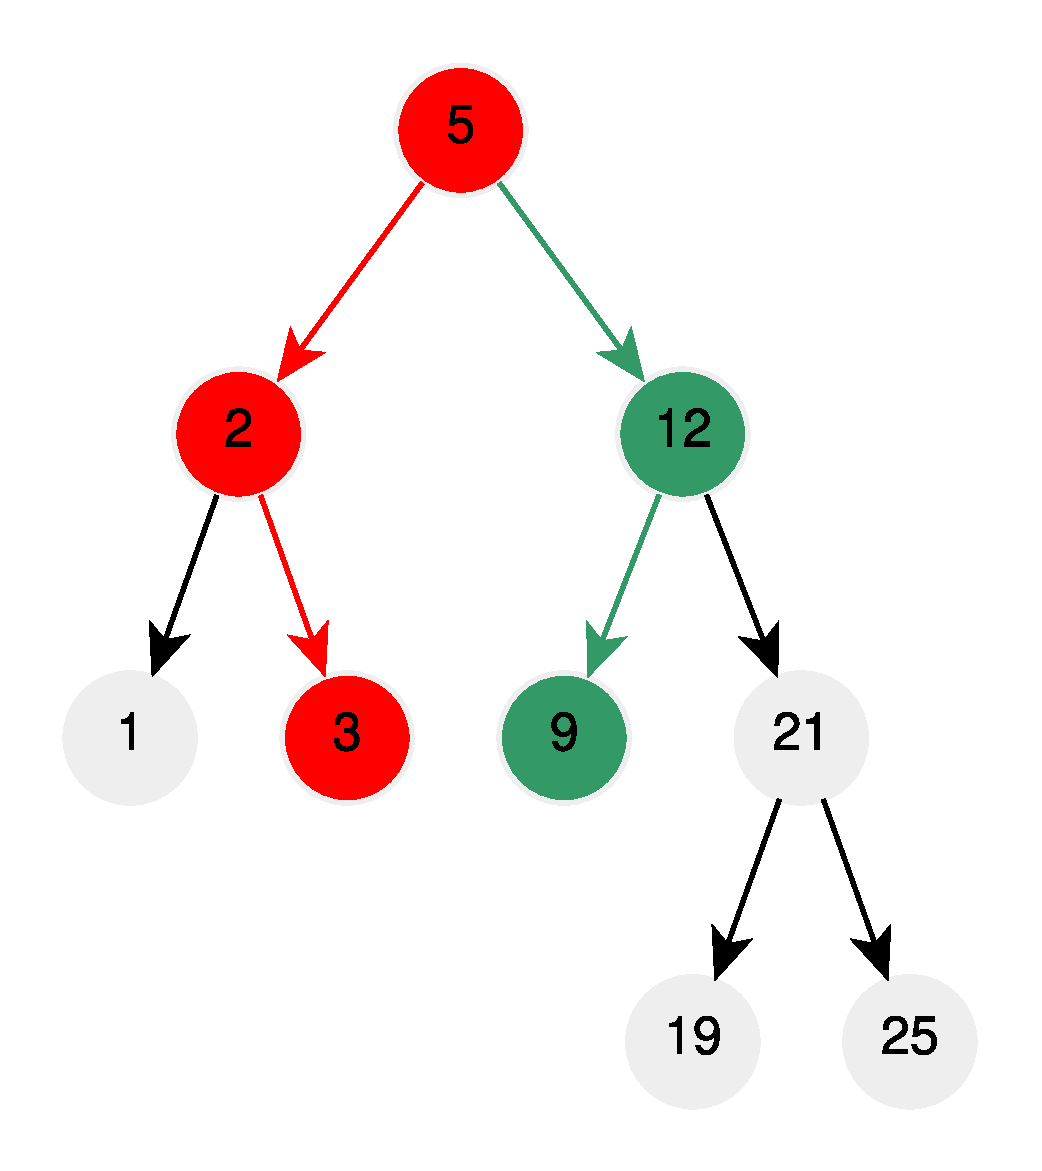
\includegraphics[scale=1.0]{/home/dspataro/git/algorithm_articles/sources/trapping_water/images/example3}
		\caption{This figure shows how the contribution of a single element of the histogram can be calculated using the information about the highest bar on its left and right.}
\end{figure}

To summarize, we can calculate the answer to this problem by:
\begin{enumerate}
	\item For each element of the array \inline{H[i]}
	\item calculate the highest bar on its left \inline{b_l} and the highest bar on its right \inline{b_r}.
	\item add \inline{std::max(0, std::min(b_l, b_r) - H[i])}
\end{enumerate}

Step $2$ of this approach can be implemented with a simple linear search with a cost of $O(n)$ making the complexity of whole algorithm equal to $O(n^2)$. Finding the maximum elements on left and right costs has a linear complexity, and it needs to be done for all the bars.
Moreover note that the first and the last element will never be able to contain any water as those elements have no bars on their left and right, respectively.

Listing \ref{list:trapping_water:bruteforce} shows a possible implementation of this idea. Note how the \inline{std::max_element} function from C++ STL can be employed elegantly to calculate $b_l$ and $b_r$.

\lstinputlisting[language=c++, caption=Brute-force solution to the problem of calculating the amount of water trapped between buildings.,label=list:trapping_water:bruteforce]{/home/dspataro/git/algorithm_articles/sources/trapping_water/trapping_water_solution1.cpp}



\subsection{Dynamic Programming}
\label{trapping_water:sec:dp}
The solution proposed in Section \ref{trapping_water:sec:bruteforce} is far from optimal, but it can be transformed into a good one, if we realize that
for each element of the array, we can calculate and \textbf{store} the values for its max element on its right and on its left. As already discussed in Chapter \ref{ch:greatest_right}, this task can be accomplished in linear time. Thus all it is necessary is to keep two additional arrays, $R$, and $L$, of  length $n$ (same length of the input). 

\begin{itemize}
	\item $R[i]$ contains the value of the highest bar among all elements of the input with index $j > i$ (on the right of, and not considering, $i$).
	\item symmetrically, $L[i]$ contains the value of the highest bar among all elements of the input with index $j < i$ (on the left of, and not considering, $i$).
\end{itemize}

Armed with this information, the same algorithm used in the Section \ref{trapping_water:sec:bruteforce} can be turned into an elegant and efficient solution that will make any interviewer happy. Listing \ref{list:trapping_water:dp} shows a possible implementation of this idea. Note that we can calculate $R$, given a function, \inline{max_left} that is able to calculate $L$, by simply providing its input reversed and reversing the results once again. This is how $R$ is calculated in Listing \ref{list:trapping_water:dp}.

Figures \ref{fig:trapping_water_DPL} and \ref{fig:trapping_water_DPR} show a representation of $L$ and $R$. As we can see in Figure \ref{fig:trapping_water_DPLR} the amount of trapped water can be visualized by superimposing the two figures and taking the intersection of the shadowed cells.


\begin{figure}
\centering
\begin{subfigure}[b]{0.95\textwidth}
   \includegraphics[width=1\linewidth]{/home/dspataro/git/algorithm_articles/sources/trapping_water/images/DPR}
   \caption{Representation of the highest value on the right of each element. A cell colored in \textcolor[HTML]{3268d5}{$\blacksquare$} have at least a pile with height higher or equal to the cell itself on its \textbf{right}. }
   \label{fig:trapping_water_DPL}
\end{subfigure}

\begin{subfigure}[b]{0.95\textwidth}
   \includegraphics[width=1\linewidth]{/home/dspataro/git/algorithm_articles/sources/trapping_water/images/DPL}
   \caption{Representation of the highest value on the right of each element. A cell colored in \textcolor[HTML]{32d579}{$\blacksquare$} have at least a pile with height higher or equal to the cell itself on its \textbf{left}.}
   \label{fig:trapping_water_DPR}
\end{subfigure}

\begin{subfigure}[b]{0.95\textwidth}
   \includegraphics[width=1\linewidth]{/home/dspataro/git/algorithm_articles/sources/trapping_water/images/DPLR}
   \caption{Superimposition of Figures \ref{fig:trapping_water_DPL} and \ref{fig:trapping_water_DPR}. Cells colored in \textcolor[HTML]{5aa1c7}{$\blacksquare$} represent the intersection between cells colored in \textcolor[HTML]{3268d5}{$\blacksquare$} in Figure \ref{fig:trapping_water_DPL} and cells colored in \textcolor[HTML]{32d579}{$\blacksquare$} in Figure \ref{fig:trapping_water_DPR}. Those cells are the ones that can be filled up with water.}
   \label{fig:trapping_water_DPRL}
\end{subfigure}

\end{figure}


\lstinputlisting[language=c++, caption={Dynamic programming, $O(n)$ time and space, solution to the problem of calculating the amount of water trapped between buildings.},label=list:trapping_water:dp]{/home/dspataro/git/algorithm_articles/sources/trapping_water/trapping_water_solution2.cpp}

This solution has a time complexity of $O(n)$ because the computation of $L$ and $R$ can be done in linear time, while calculating the final answer can be done in a single pass over the array. The space complexity if linear as well because the arrays $L$ and $R$ are both of size proportional to the size of $n$.


\subsection{Two pointers solution}
\label{trapping_water:sec:two_pointers}
Despite the fact that the solution presented in Section \ref{trapping_water:sec:dp} is already a good one, we can definitely do better and lower the space complexity down to $O(1)$. The key idea is that, we do not really need to store $L$ and $R$ in their entirety. All of time, we only need one element from both $L$ and $R$ and nothing else. Once an element of the input array is processed we can discard the corresponding element in $L$ and $R$ because they are of no use anymore in the future. They do not play a role in the calculation of any other element of the input array $H$. Therefore the solution proposed in this section will use a two pointer technique and will keep two \textit{rolling} maximum value $m_l$ and $m_r$, one for the left and one for the right. When processing the cell at index $i$ of the input array, $m_l$ and $m_r$ will contain the maximum value on the left  and on the right of $i$, respectively.

The input arrays is traversed from left to right using two pointers $l$ and $r$, pointing at first to the beginning and the end of the input array.$m_l$ and $m_r$ are set to $0$ respectively. At each iteration only one of the two pointers is moved towards the center depending on whether \inline{H[i] <= H[j]} is:
\begin{description}
\item[true]  then the contribution of \inline{H[i]} is bounded by \inline{m_l} (because \inline{H[r] >= H[l]}. the left pointer is moved towards the center (we have considered the contribution of this cell and we can move forward).\\
\item[false] then the contribution of \inline{H[j]} is bounded by \inline{m_r} (because \inline{H[l] > H[r]}. The right pointer is moved towards the center (we have considered the contribution of this cell and we can move forward). \\
\end{description}

While moving the pointers the variables $m_l$ or $m_r$ are updated and the contribution of every single element summed up.

An implementation of the idea above is shown in Listing \ref{list:trapping_water:two_pointers}. Note that all the elements of the input array will be eventually considered because $l$ and $r$ are moved one by one against each other. 

\lstinputlisting[language=c++, caption={Two pointers solution, $O(n)$ time and  $O(1)$ space, solution to the problem of calculating the amount of water trapped between buildings.},label=list:trapping_water:two_pointers]{/home/dspataro/git/algorithm_articles/sources/trapping_water/trapping_water_solution3.cpp}

This approach has a time complexity of $O(n)$ (we cannot do better than this because at least we have to touch all the elements of the input at least once) and a space complexity of $O(1)$. This is therefore the optimal approach to solve this problem  and we believe this should be your solution during an actual interview.


\subsection{Stack based solution}
\label{trapping_water:sec:stack}
There is another way of solving this problem that uses an additional stack. At any moment the stack will contains indexes of bars that are bounded on the left by some other bar. It means that the stack will contain bars in a decreasing order (from the bottom to the top). The idea is that we start with an empty stack $S$ and iterate thought the input array from start to end, and for each bar $b_i$:
we check whether it is lower than the top of the stack $S_{top}$. If that is the case, the current top of the stack is higher than this element and so it means that the current top bounds the current element from the left. In this case we simply add it to the  top of the stack. If it not the case then we have a bar that is higher or equal to the top. Thus  all the bars in the stack that are smaller or equal of $i$ can trap some water because they are bound from left (by other taller elements in the stack) and to the right by $i$ itself.
Given the stack $S=[s_0, s_1,s_2]$ where $s_0 \geq s_1 \geq s_2$ (remember they are increasing from top to bottom) we know that we can use bar $i$ and bar $s_1$ to calculate the contribution of $s_2$ to the final answer and we can use bar $i$ and bar $s_0$ to calculate the contribution of $s_1$. The contribution of each element is calculated as the rectangle of base equal to the distance between the two bounding bars and height that is equal to the minimum of the heights between the two bounding bars \textbf{minus} the height of the bar we are calculating the contribution. 

A possible implementation of this idea is shown in Listing \ref{list:trapping_water:stack}. Note how all the real work happens inside the \inline{while} loop and that the bar we calculate the contribution is named top while the bar on the left and right are named \inline{bar_left} and \inline{bar_right} respectively. Moreover, no matter the stack is unwounded or not the \inline{bar_right} is \textbf{added} to the stack because when controls reaches line $21$ it will be either the only bar in the stack of it will be smaller than the current top.


\lstinputlisting[language=c++, caption={Stack based solution, $O(n)$ time and  space, solution to the problem of calculating the amount of water trapped between buildings.},label=list:trapping_water:stack]{/home/dspataro/git/algorithm_articles/sources/trapping_water/trapping_water_solution4.cpp}